\providecommand{\main}{../../../..}
\documentclass[\main/dresen_thesis.tex]{subfiles}

\begin{document}
  \label{sec:monolayers:nanoparticle:xrd}
  \begin{figure}[tb]
    \centering
    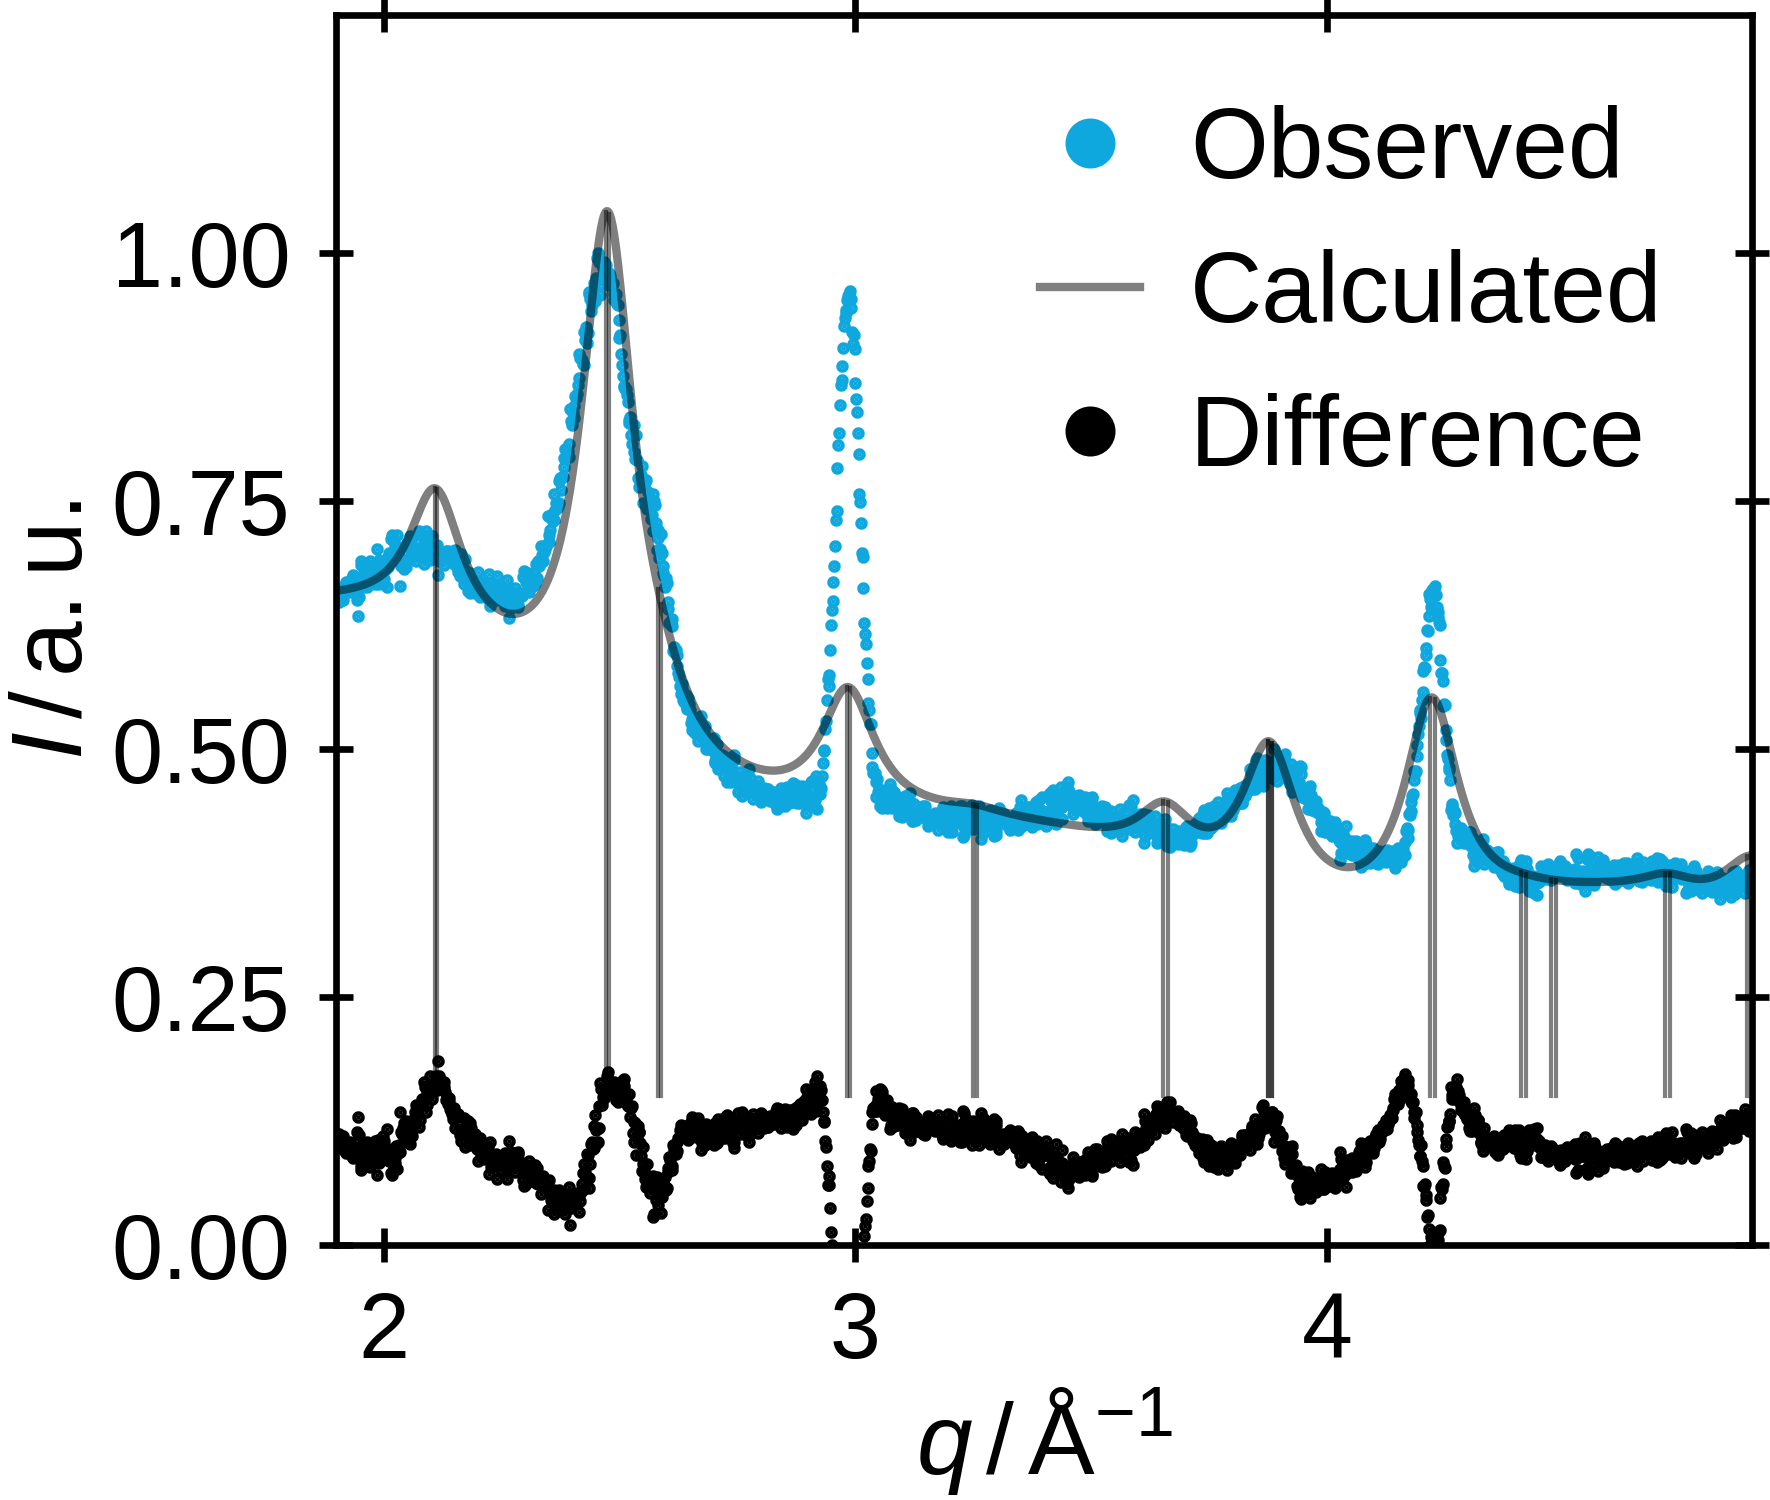
\includegraphics{monolayer_XRD_Ol_CoFe_C}
    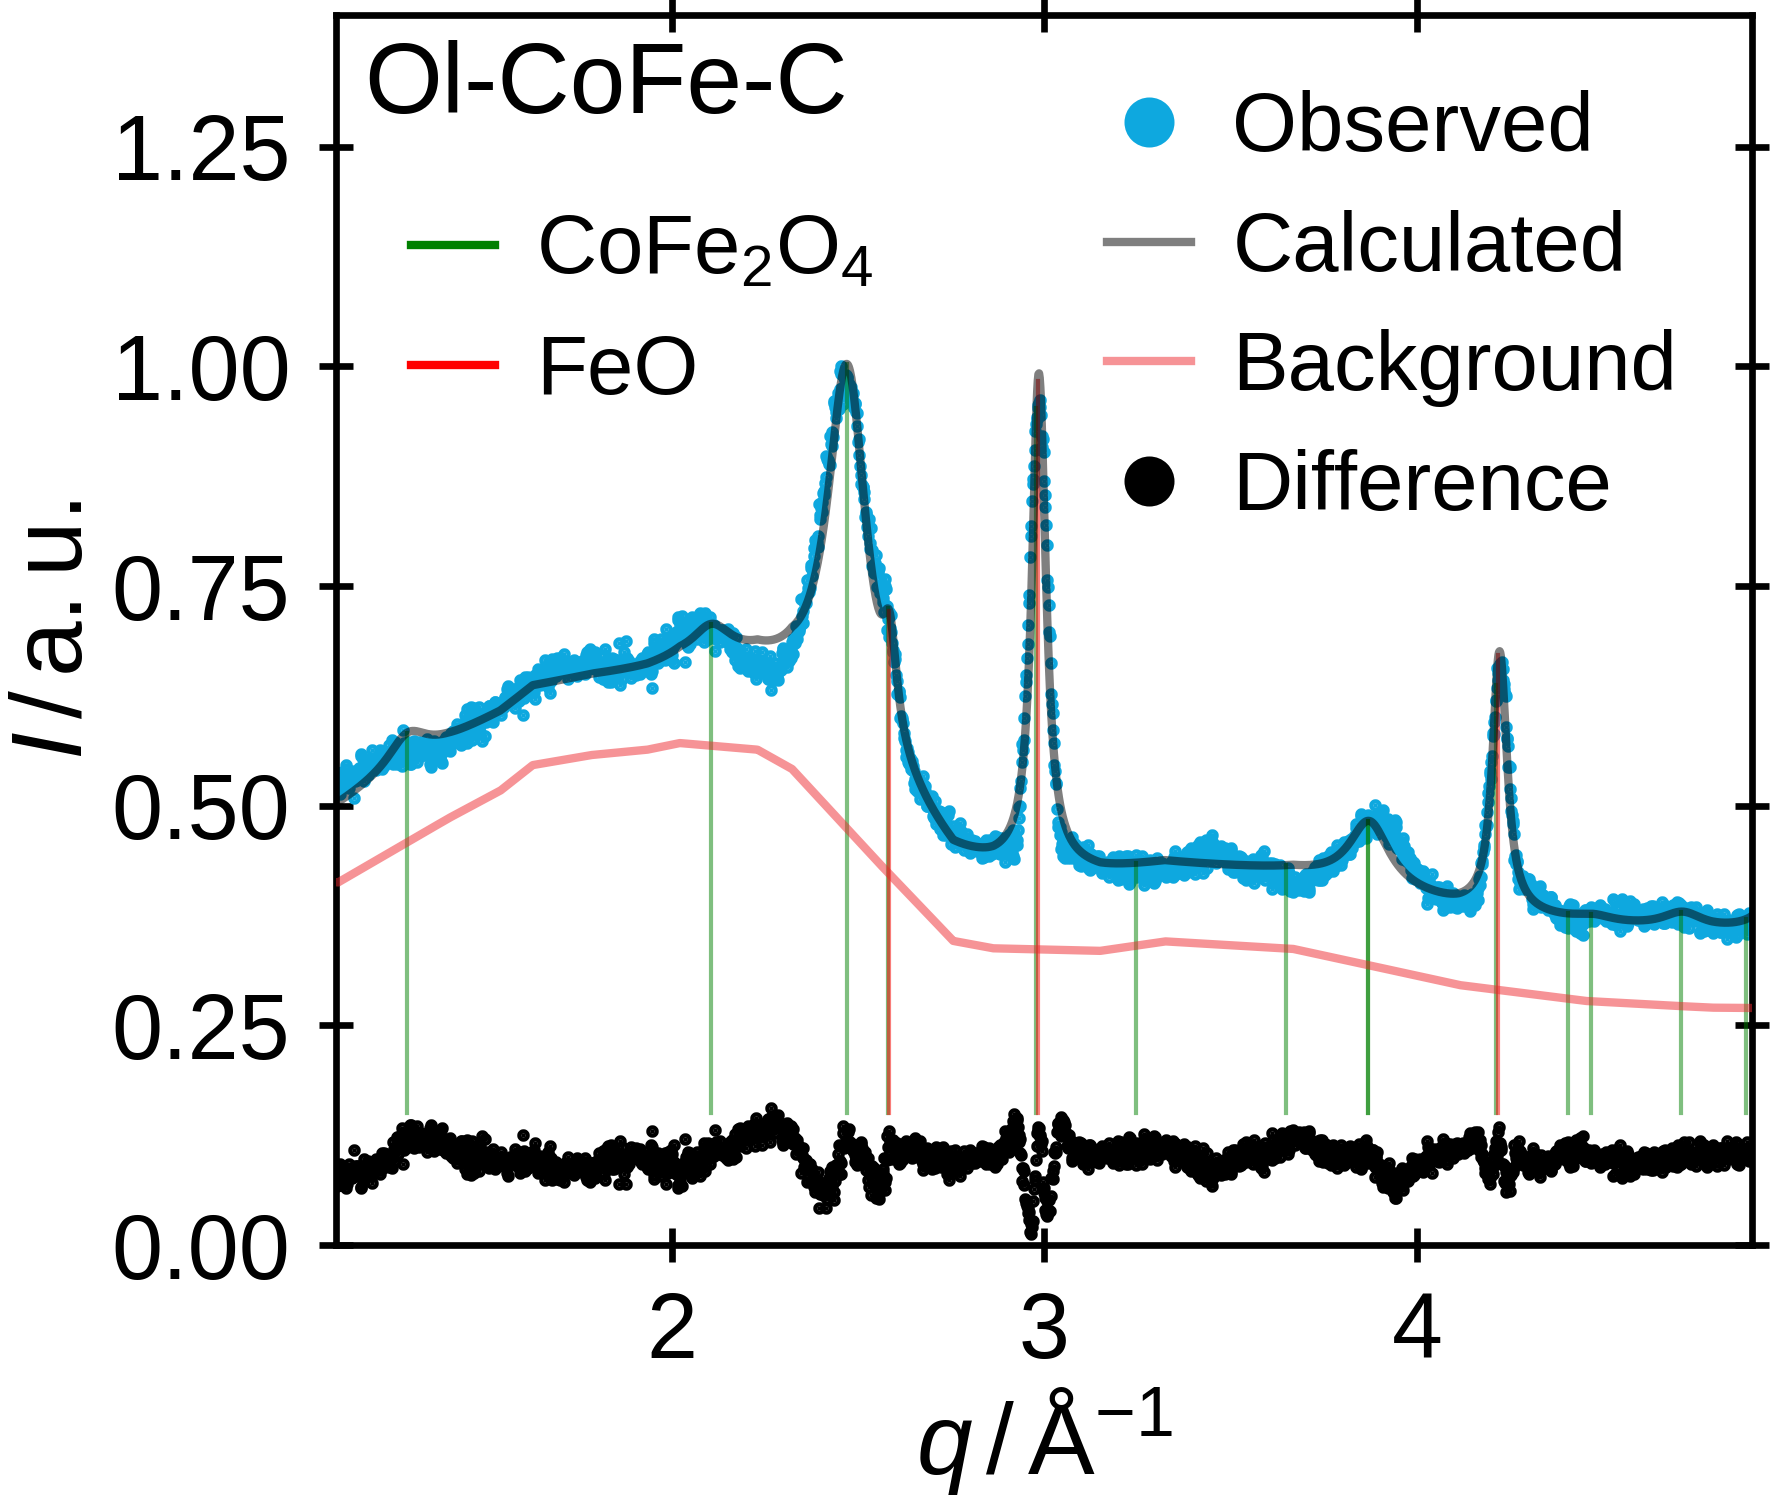
\includegraphics{monolayer_XRD_CoFe2O4WustiteFit_Ol_CoFe_C}
    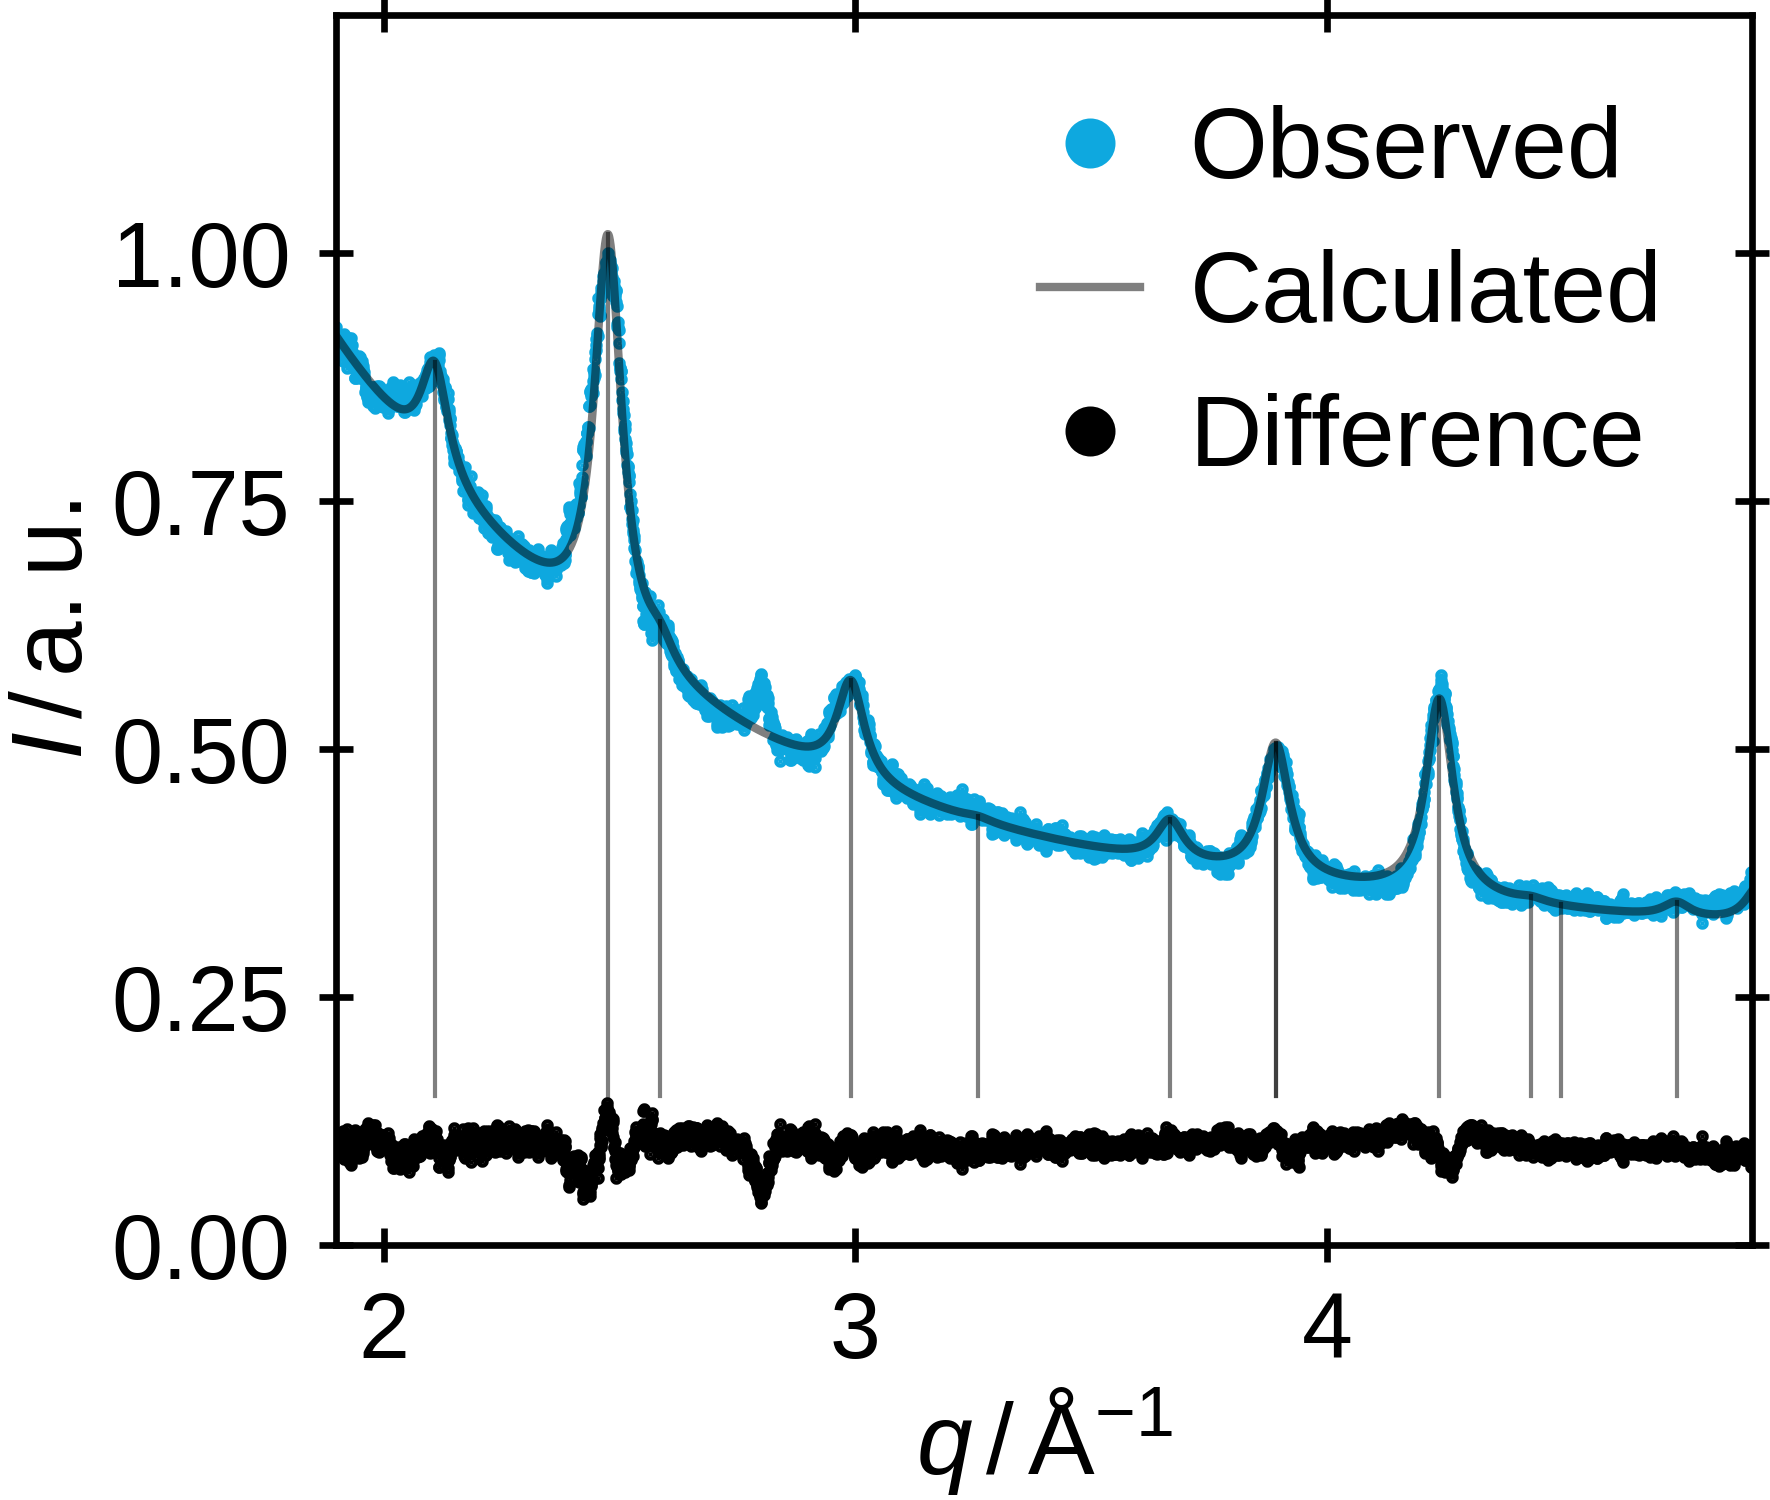
\includegraphics{monolayer_XRD_Ac_CoFe_C}
    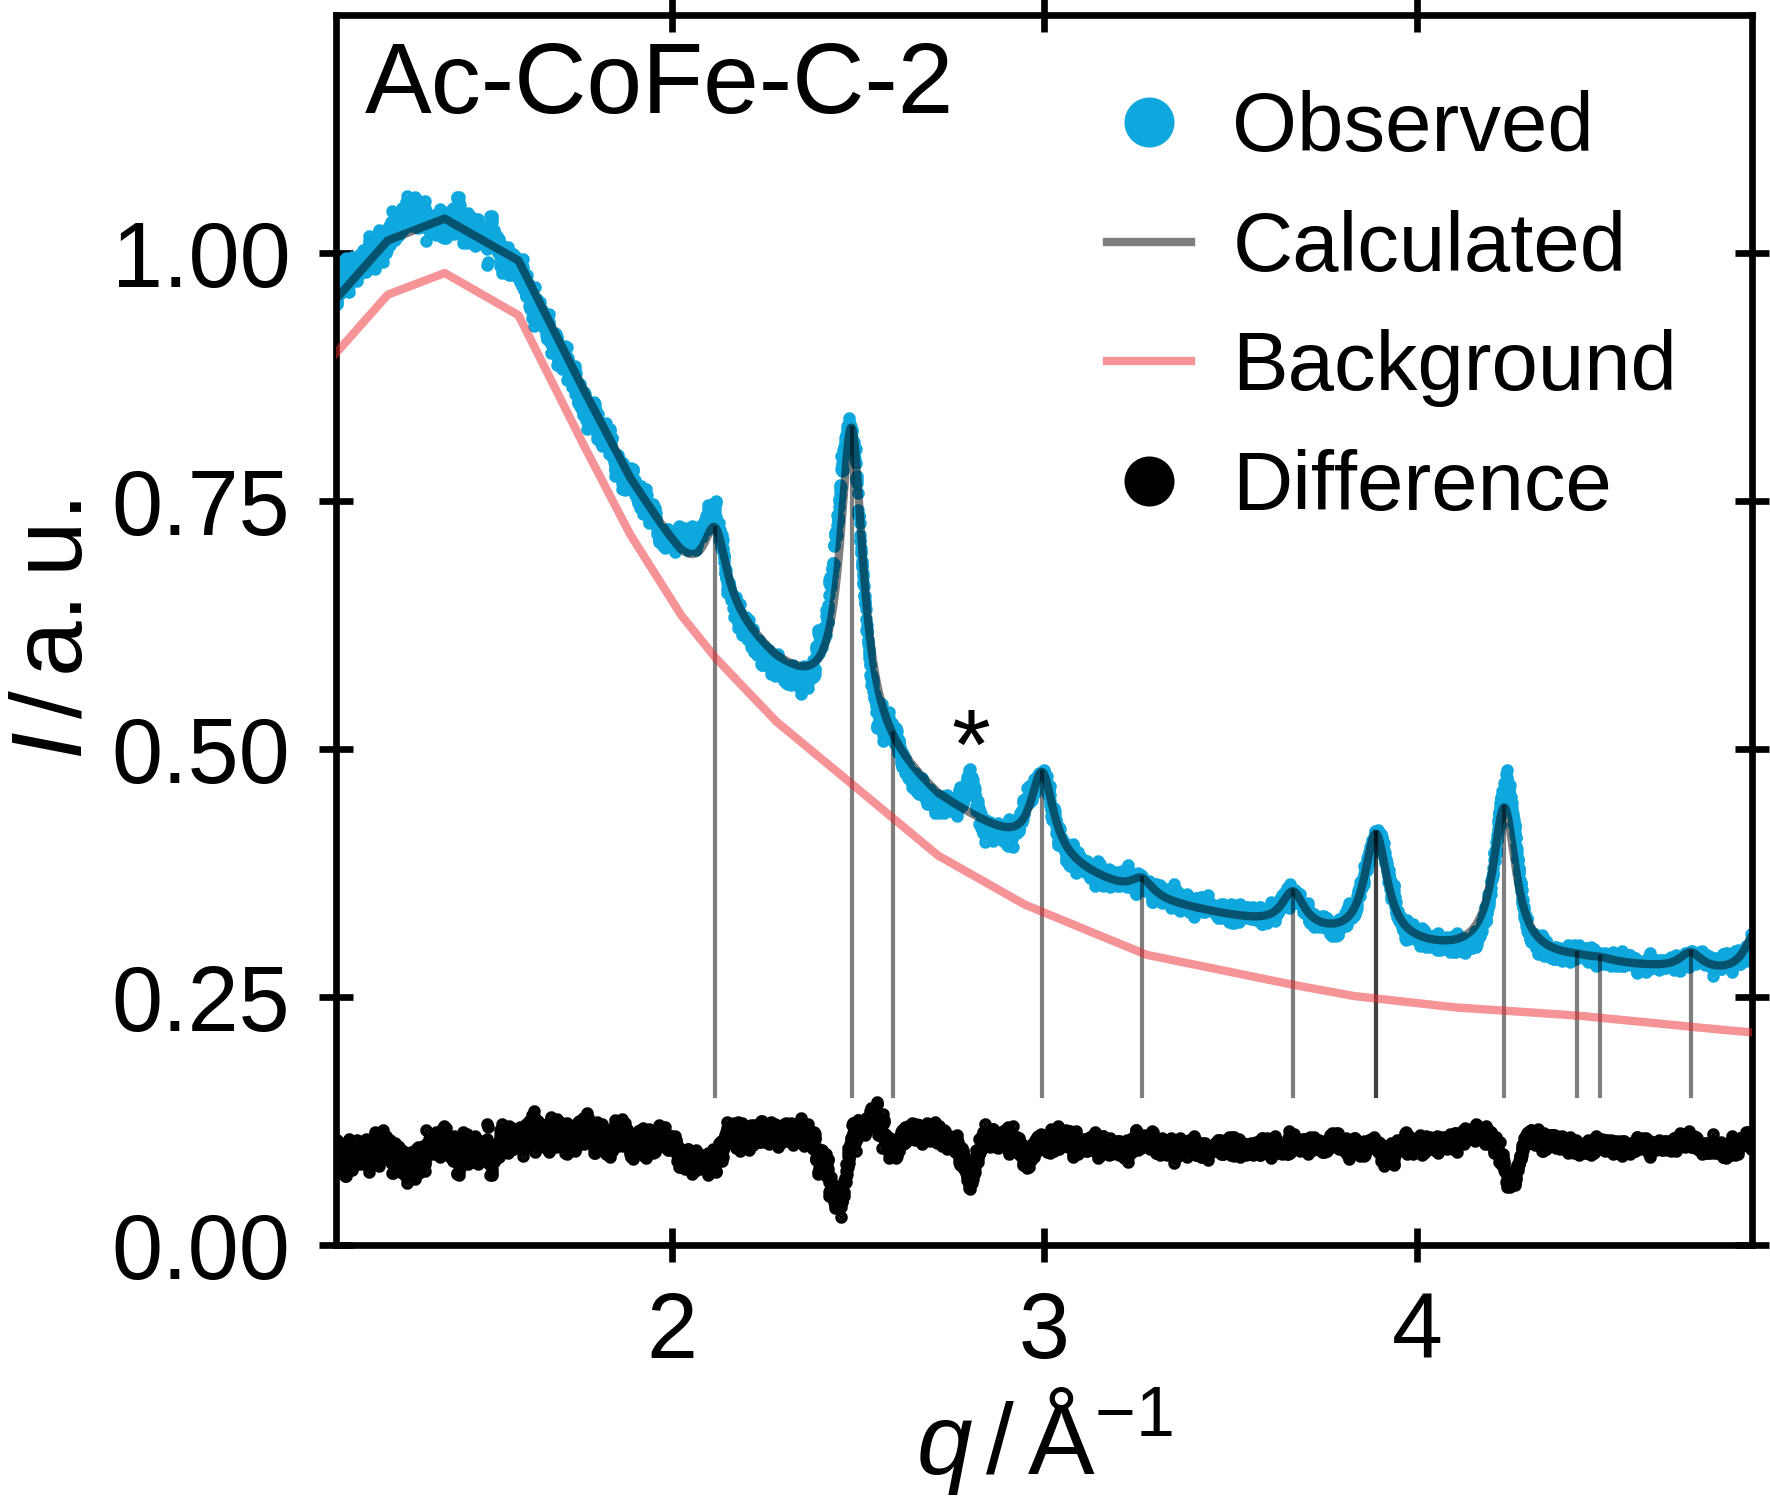
\includegraphics{monolayer_XRD_Ac_CoFe_C_2}
    \caption{\label{fig:monolayers:nanoparticle:xrd}X-ray diffraction of Ol-CoFe-C with a LeBail fit of only a \ch{CoFe2O4} phase (upper left) and a fit with two phases, namely \ch{CoFe2O4} and \ch{FeO} (upper right). The lower XRD show Ac-CoFe-C (lower left) and Ac-CoFe-C-2 (lower right) both with a LeBail fit of a \ch{CoFe2O4} phase. The red curve shows in each case the manually selected background.}
  \end{figure}

  Diffraction data shown in \reffig{fig:monolayers:nanoparticle:xrd} for the three nanoparticle batches is evaluated by a LeBail fit of the phase to check for phase purity, as well as to determine the lattice constant and the average crystallite size of the particles.
  The nanoparticles prepared from acetylacetonates are well described by the space group of the inverse spinell.
  The resulting parameters of the LeBail fits, namely the lattice constants $a$ and the Lorentzian broadening $Y$ of the peaks are listed for all four LeBail fits in \reftab{tab:monolayers:nanoparticle:discussion:xrdLeBail}.

  The LeBail fit of Ol-CoFe-C is not well described by the single \ch{CoFe2O4} as especially the peak at $q \eq 3 \unit{\angstrom^{-1}}$ has a smaller broadening.
  By adding a w\"ustite phase to the LeBail fit as suggested by literature \cite{Bodnarchuk_2009_Excha}, the diffractogram can however be completely described.
  In the data set of Ac-CoFe-C-2 a single reflex that does not fit to the phase is visible and marked by an asterisk (*).
  This data set was measured at another diffractometer than the other two nanoparticle batches, and after consulting with the instrument responsible, he confirmed that this peak is commonly observed in the instrumental setup and does not originate from the sample.
  \begin{table}[ht]
    \centering
    \caption{\label{tab:monolayers:nanoparticle:discussion:xrdLeBail}Parameters of LeBail fit for Ac-CoFe-C and Ac-CoFe-C-2 with the inverse spinell phase of \ch{CoFe2O4}, as well as the results of the LeBail fit for Ol-CoFe-C using once the \ch{CoFe2O4} phase and once a combination of \ch{CoFe2O4} and a W\"ustite phase. The parameters for each phase are $a$ the respective lattice constant and $Y$ the Lorentzian isotropic size parameter. The calculate crystallite size $L$ is given for each lattice, as well as the wavelength $\lambda$ used at each measurement, the figure of merit $\chi^2$ and the agreement factors $R$.}
    \begin{tabular}{ l | l | l }
      \hline
      \rule{0pt}{2ex}                                 & \textbf{Ac-CoFe-C} & \textbf{Ac-CoFe-C-2} \\
      \hline
      \rule{0pt}{2ex}space group & \multicolumn{2}{c}{$Fd\bar{3}m$ (No. 227)} \\
      \hline
      \rule{0pt}{2ex} $a \,/ \unit{\angstrom}$        & $8.3949(2)$        & $8.3938(1)$\\
      \rule{0pt}{2ex} $Y \,/ \unit{^\circ}$           & $1.063(3)$         & $0.438(1)$ \\
      \hline
      \rule{0pt}{2ex} $L \,/ \unit{nm}$               & $5.285(3)$         & $5.916(5)$ \\
      \hline
      \rule{0pt}{2ex} $\lambda \,/ \unit{\angstrom}$  & $1.54056$          & $0.71070$ \\
      \hline
      \rule{0pt}{2ex} $\chi^2$                        & $1.68$             & $1.40$ \\
      \rule{0pt}{2ex} $R_p \,/ \unit{\%}$                           & $2.06$             & $1.85$ \\
      \rule{0pt}{2ex} $R_{wp} \,/ \unit{\%}$                        & $2.63$             & $2.69$ \\
      \rule{0pt}{2ex} $R_{exp} \,/ \unit{\%}$                       & $2.03$             & $2.28$ \\
      \rule{0pt}{2ex} $R_{f} \,/ \unit{\%}$                         & $0.24$             & $0.05$ \\
      \hline
      \hline
      \rule{0pt}{2ex} & \multicolumn{2}{c}{\textbf{Ol-CoFe-C}}\\
      \hline
      \hline
      \rule{0pt}{2ex}space group & $Fd\bar{3}m$ (No. 227) & + $Fm\bar{3}m$ (No. 225)\\
      \hline
      \rule{0pt}{2ex} $a_\mathrm{inv. spinell} \,/ \unit{\angstrom}$         & $8.4309(3)$ & $8.4384(4)$  \\
      \rule{0pt}{2ex} $Y_\mathrm{inv. spinell} \,/ \unit{^\circ}$            & $1.126(7)$  & $1.798(8)$   \\
      \rule{0pt}{2ex} $a_\textsf{w\"ustite}     \,/ \unit{\angstrom}$        &             & $4.2125(1)$  \\
      \rule{0pt}{2ex} $Y_\textsf{w\"ustite}     \,/ \unit{^\circ}$           &             & $0.575(3)$   \\
      \hline
      \rule{0pt}{2ex} $L_\mathrm{inv. spinell} \,/ \unit{nm}$                & $4.990(3)$  & $3.124(1)$ \\
      \rule{0pt}{2ex} $L_\textsf{w\"ustite}      \,/ \unit{nm}$              &             & $9.767(3)$ \\
      \hline
      \rule{0pt}{2ex} $\lambda \,/ \unit{\angstrom}$  & \multicolumn{2}{c}{$1.54056$}\\
      \hline
      \rule{0pt}{2ex} $\chi^2$                                               & $7.87$      & $2.51$ \\
      \rule{0pt}{2ex} $R_p \,/ \unit{\%}$                                                  & $3.58$      & $2.33$ \\
      \rule{0pt}{2ex} $R_{wp} \,/ \unit{\%}$                                               & $5.28$      & $2.99$ \\
      \rule{0pt}{2ex} $R_{exp} \,/ \unit{\%}$                                              & $1.88$      & $1.88$ \\
      \rule{0pt}{2ex} $R_{f, \, \mathrm{inv. spinell}} \,/ \unit{\%}$                      & $0.48$      & $0.46$ \\
      \rule{0pt}{2ex} $R_{f, \, \text{w\"ustite}} \,/ \unit{\%}$                           &             & $0.29$ \\
      \hline
    \end{tabular}
  \end{table}

  \paragraphNewLine{Lattice constant}
    Both acetylacetonate nanoparticle batches show a similar lattice constant, with $8.3949(2) \unit{\angstrom}$ for Ac-CoFe-C and $8.3938(1) \unit{\angstrom}$ for Ac-CoFe-C-2.
    Both are only slightly larger but close to the lattice constant reported for bulk cobalt ferrite $a_\mathrm{bulk} \eq 8.3919 \unit{\angstrom}$ \cite{Stein_2018_Struct}.
    For Ol-CoFe-C, the cobalt ferrite lattice constant obtained by the LeBail fit with two phases is $8.4384(4) \unit{\angstrom}$ and thereby larger in comparison with the bulk the acetylacetonate particles and the bulk value.
    On the other hand, the lattice constant for the W\"ustite phase is with $4.2125(1) \unit{\angstrom}$ in comparison to the bulk values of FeO ($a_\mathrm{FeO} \eq 4.33 \unit{\angstrom}$ \cite{Hentschel_1970_Stoich}) and CoO ($a_\mathrm{CoO} \eq 4.26 \unit{\angstrom}$) both smaller.
    While no discussion of the compression of the w\"ustite lattice could be found in literature for cobalt ferrite particles prepared from oleates, the compression is observed for core-shell iron oxide/w\"ustite nanoparticles from iron oleate  \cite{Wetterskog_2013_Anoma}.
    Here, it is explained that the compression is a result of the lattice mismatch.
    This can also be applied in this case where the lattice constant of the inverse spinell is very close to being two times the lattice constant of the w\"ustite phase.

  \paragraphNewLine{Crystallite Size}
    The Lorentzian peak broadening for Ac-CoFe-C, which was measured on a Cu-K$\alpha$ source, corresponds to a crystallite size of $5.285(3) \unit{nm}$.
    For Ac-CoFe-C-2, which was measured on a Mo-K$\alpha$ source, the broadening corresponds to a crystallite size of $5.916(5) \unit{nm}$.
    For Ol-CoFe-C two broadening parameters are obtained, one for the inverse spinell phase, which corresponds to $L_{\mathrm{inv. spinell}} \eq 3.124 \unit{nm}$, and one for the w\"ustite phase which corresponds to $L_{\textsf{w\"ustite}} \eq 9.767 \unit{nm}$.

    In the case of the acetylacetonate particles, the obtained values of the average crystallite sizes determined by XRD are smaller than the average particle size that is obtained by TEM ($10.1 \unit{nm}$ and $10.8 \unit{nm}$ for Ac-CoFe-C and Ac-CoFe-C-2 respectively).
    For Ac-CoFe-C-2 the underestimation of the crystallite size could be argued with due to the missing instrumental resolution reference, however for Ac-CoFe-C this is corrected for.
    This points to an additional broadening of the peaks additionally to the finite-size effect, as possibly imperfect crystalline order, which results in disorder of the second kind.

    For Ol-CoFe-C, the individual crystallite sizes are smaller than the total particle size from TEM ($10.9 \unit{nm}$), but the combined size of the two crystallite sizes ($12.891 \unit{nm}$) is $18 \%$ larger in comparison.

    % From the crystallite sizes it can be deduced that the wustite phase dominates the volume of the particle as
    % \begin{align}
    %   \frac{V_{\textsf{w\"ustite}}}{V_{\textsf{w\"ustite}} + V_{\mathrm{inv. spinell}}} \eq \frac{L^3_{\textsf{w\"ustite}}}{ L^3_{\textsf{w\"ustite}} + L^3_{\mathrm{inv. spinell}}} \eq 96.8 \%.
    % \end{align}
\end{document}